%-------------------------------------------------------------------------------
\documentclass[twocolumn]{article}

%-------------------------------------------------------------------------------
% Packages
\usepackage[portuguese]{babel}
\usepackage{booktabs}
\usepackage{environ}
\usepackage[margin=2cm]{geometry}
\usepackage{graphicx}
\usepackage{hyperref}
\usepackage{minted}
\usepackage{xcolor}

%-------------------------------------------------------------------------------
% Project configs
\title{Relatório de I.A.: Sistemas Fuzzy (Trabalho 4)}
\author{Cauê Baasch de Souza \\
        João Paulo Taylor Ienczak Zanette}
\date{\today}

%-------------------------------------------------------------------------------
\begin{document}
    \maketitle{}

    \section{O ``Fuzzy Truck''}

    No problema ``Fuzzy Truck'', é necessário definir parâmetros, saídas e
    regras de um sistema Fuzzy para fazer um caminhão, andando de ré,
    estacionar em uma doca considerando um espaço 2D sem obstáculos. Como
    restrições do problema, o caminhão possui velocidade constante (com exceção
    de que ele para quando está suficientemente próximo do espaço que delimita
    a vaga) e suas únicas ações possíveis são: girar o volante para a esquerda
    (indicado pelo valor -1), manter a direção atual do caminhão (valor 0) e
    girar o volante para a direita (valor 1).

    O espaço por onde o caminhão anda é delimitado pelas coordenadas X e Y
    variando de 0 a 1 com um pequeno limiar extra (com exceção de valores de $Y
    > 1$). Ao se passar dessa delimitação, a simulação é encerrada e uma
    pontuação é dada considerando o número de passos dados, o ângulo final do
    caminhão e a distância até a doca, que está centralizada no ponto $(0.5,
    1)$.

    Para simulação, é utilizado um programa gráfico simples
    (Figura~\ref{simulator}), escrito em Java, que simula o sistema em duas
    instâncias. O objetivo é que cada instância represente um competidor, que
    irá rodar seu sistema de inferência Fuzzy e enviar comandos ao programa. A
    comunicação é feita via Sockets em um host e portas pré-definidos
    (\texttt{localhost} para o Host, e 4321 e 4322 para as portas de cada
    jogador). Todo o código da solução realizada neste trabalho está disponível
    em~\cite{oficial-repo}. Nele, um arquivo ``readme.md'' descreve os
    principais arquivos a serem analisados para a implementação desta solução.

    \begin{figure}[ht]
        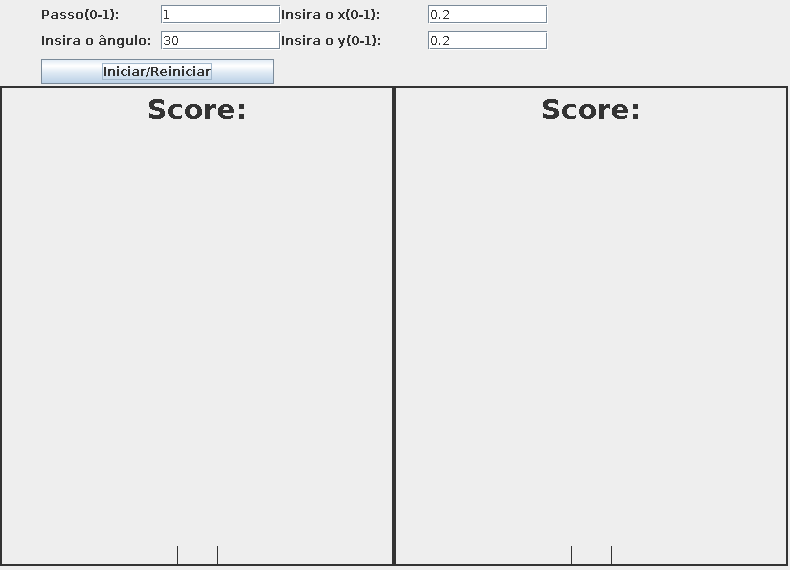
\includegraphics[keepaspectratio,width=.5\textwidth]{img/fuzzytruck-initial}
        \caption{Tela inicial do simulador para o Fuzzy Truck.\label{simulator}}
    \end{figure}

    \section{Resolvendo o problema do ``Fuzzy Truck''}

    \subsection{Entradas utilizadas e Conjuntos Fuzzy}

    Foram utilizadas três entradas simples, descritas na
    Tabela~\ref{system-entries}, em que X e Y simbolizam as coordenadas do
    caminhão.

    \begin{table}[ht]
        \centering{}
        \begin{tabular}{c c c c}
            \toprule
            Entrada & Símbolo & Tipo & Intervalo esperado \\
            \midrule
            X      & \texttt{x}   & Real & $[0, 1]$ \\
            Y      & \texttt{y}   & Real & $[0, 1]$ \\
            Ângulo & \texttt{dir} & Real & $[0, 360]$ \\
            \bottomrule
        \end{tabular}
        \caption{%
            Entradas utilizadas para o sistema em questão. Cada entrada pode
            receber um valor fora de seu intervalo esperado, porém o
            comportamento resultante não pode ser previsto nesse
            caso.\label{system-entries}
        }
    \end{table}

    Os conjuntos fuzzy (visualizáveis na Figura~\ref{fuzzy-sets}) foram
    definidos pensando em:

    \begin{itemize}
        \item O quão longe o caminhão está horizontalmente, separando em:
            ``muito para a esquerda'', ``muito para a direita'' e
            ``centralizado'';
        \item O quão longe o caminhão está verticalmente, separando em: ``muito
            longe'' e ``próximo'';
        \item A direção da traseira do caminhão, separada em: norte, sul, leste
            e oeste.
    \end{itemize}

    \begin{figure}[ht]
        \centering{}
        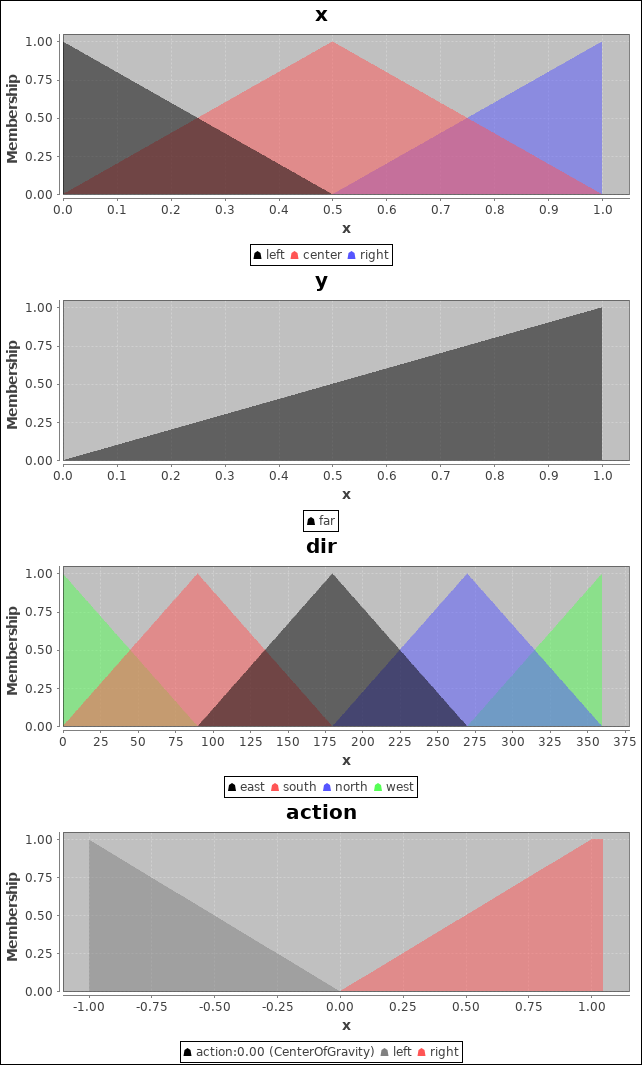
\includegraphics[keepaspectratio,width=.5\textwidth]{img/truck-fuzzifiers}
        \caption{%
            Conjuntos Fuzzy para variáveis de entrada e saída do ``Fuzzy
            Truck''.\label{fuzzy-sets}
        }
    \end{figure}

    \subsection{Regras utilizadas e Defuzzificação}

    O sistema modelado dá como saída uma variável chamada de ``Ação''
    (\texttt{action} na Figura~\ref{fuzzy-sets}), que pode ser:

    \begin{itemize}
        \item Virar o volante para a direita (valores de -1 a 0);
        \item Virar o volante para a esquerda (valores de 0 a 1);
    \end{itemize}

    Por consequência da inferência do sistema Fuzzy, ``0'' corresponde a ``Não
    virar''. Anteriormente havia sido definido um intervalo específico para
    essa ação, centralizado em ``0'', porém ele se mostrou desnecessário e
    ineficiente, porque uma decisão que deveria ter um alto grau de pertinência
    para ``Não virar'' já terá, de acordo com as regras, um baixo grau de
    pertencimento aos conjuntos respectivos às outras ações. Consequentemente,
    tal decisão já terá um valor próximo do zero esperado.

    Por simplicidade, as regras definidas foram:

    \begin{itemize}
        \item Muito para a esquerda $\land$ Norte $\rightarrow$ Virar para a
            direita
        \item Muito para a esquerda $\land$ Muito longe $\land$ Leste
            $\rightarrow$ Virar para a direita
        \item Muito para a esquerda $\land$ Muito longe $\land$ Sul
            $\rightarrow$ Virar para a esquerda
        \item Centralizado $\land$ Oeste $\rightarrow$ Virar para a esquerda
        \item Centralizado $\land$ Norte $\rightarrow$ Virar para a esquerda
        \item Centralizado $\land$ Leste $\rightarrow$ Virar para a direita
        \item Muito para a direita $\land$ Norte $\rightarrow$ Virar para a
            esquerda
        \item Muito para a direita $\land$ Muito longe $\land$ Oeste
            $\rightarrow$ Virar para a esquerda
        \item Muito para a direita $\land$ Muito longe $\land$ Sul
            $\rightarrow$ Virar para a direita
    \end{itemize}

    A ação é defuzzificada dos conjuntos da saída ``Ação'' para um valor no
    intervalo $[-1, 1]$ utilizando o método do \textbf{Centro de Gravidade}.

    \section{Resultados obtidos}

    Diversos testes com diferentes valores de entrada foram feitos. Serão
    expostos aqui apenas três deles, escolhidos da forma: utilizando as
    configurações iniciais do programa de simulação
    (Figura~\ref{figure-test-default}), utilizando um caso trivial
    (Figura~\ref{figure-test-trivial}) e utilizando um \textit{corner-case}
    (Figura~\ref{figure-test-corner}). A Tabela~\ref{test-params} descreve os
    parâmetros utilizados em cada cenário.

    \begin{table}[ht]
        \centering{}
        \begin{tabular}{c c c c c c}
            \toprule
            Teste   & Passo & $X_0$ & $Y_0$ & Ângulo & Pontuação \\
            \midrule
            Padrão  & 1     & 0.2   & 0.2   & 30     & 9904.47   \\
            Trivial & 1     & 0.5   & 0.2   & 90     & 9996.00   \\
            \textit{Corner-case} & 1 & 0.8 & 0.8 & 160 & 9821.47   \\
            \bottomrule
        \end{tabular}
        \caption{%
            Parâmetros e pontuação para cada um dos casos de teste
            expostos.\label{test-params}
        }
    \end{table}

    Nos dois primeiros casos, o sistema conseguiu responder bem aos estímulos e
    levar o caminhão ao destino correto. No último, porém, a reação foi levar o
    caminhão apenas para baixo. Houveram tentativas, conforme mencionado mais à
    frente nas dificuldades encontradas para a modelagem, de resolver casos
    semelhantes com regras mais específicas (como, por exemplo, definir que
    quando o caminhão está muito próximo de $Y = 1$ deve contornar pelo outro
    lado), porém isso degradava outros resultados e nem sempre fazia o caminhão
    chegar ao seu destino.

    \begin{figure}[ht]
        \centering{}
        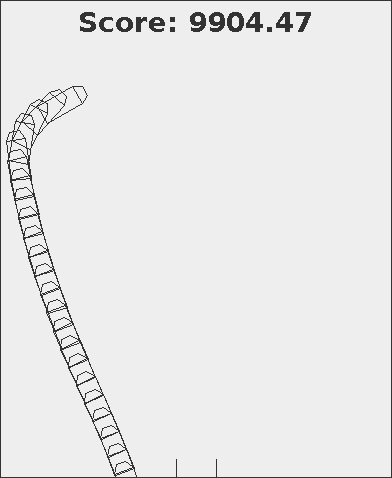
\includegraphics[keepaspectratio,width=0.25\textwidth]{img/test-default}
        \caption{%
            Trajetória do caminhão no caso padrão, utilizando as configurações
            iniciais do programa de simulação.\label{figure-test-default}
        }
    \end{figure}

    \begin{figure}[ht]
        \centering{}
        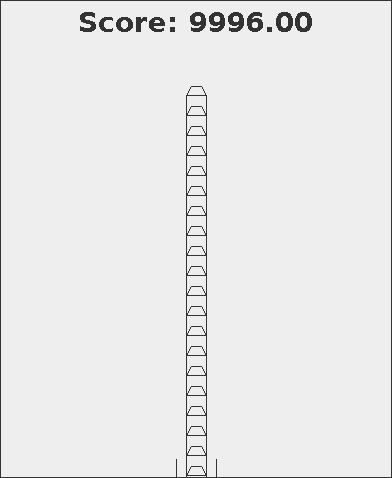
\includegraphics[keepaspectratio,width=0.25\textwidth]{img/test-trivial}
        \caption{%
            Trajetória do caminhão no caso trivial, em que o caminhão deve ir
            apenas reto.\label{figure-test-trivial}
        }
    \end{figure}

    \begin{figure}[ht]
        \centering{}
        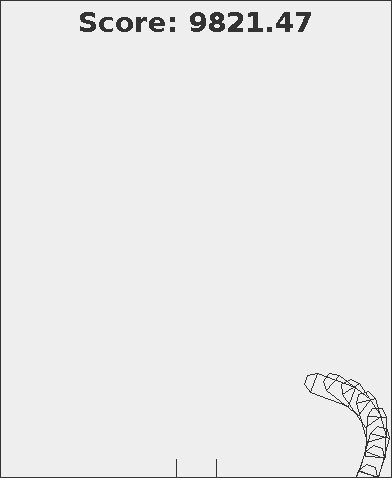
\includegraphics[keepaspectratio,width=0.25\textwidth]{img/test-corner}
        \caption{%
            Trajetória do caminhão no \textit{corner-case}. É evidente que o
            sistema não resolve esse caso.\label{figure-test-corner}
        }
    \end{figure}

    \section{Dificuldades encontradas}

    \subsection{Ferramental}

    Devido à vontade de aventura, os alunos decidiram utilizar o gerador de
    código C++ a partir de FCL (linguagem de descrição de sistemas Fuzzy) pelo
    jFuzzyLogic (biblioteca e programa para funcionalidades relacionadas a
    lógica Fuzzy, incluindo geração de gráficos). Porém, um pouco fora do
    esperado, isso acarretour na necessidade de passos extras como: melhoria do
    código gerado, separação das declarações em header, e implementação simples
    de uma API Socket em C++. Porém, tendo esses passos prontos, os ajustes e
    criação das regras e parâmetros do sistema para o FuzzyTruck foram mais
    triviais. Como FCL obriga a enumeração de regras, para melhorar a
    produtividade criou-se um pequeno script em Python que gerava o arquivo FCL
    a partir de regras definidas em uma lista de \texttt{Rule}s (uma tupla com
    os valores esperados e o valor de saída para a regra).

    \subsection{Modelagem da solução}

    Da parte da definição das regras, diferentes abordagens foram tomadas
    tentando ser o mais restritivo possível: utilização de pontos colaterais
    (totalizando 8 direções) e definindo regras para cada caso (muito longe, no
    centro ou perto em Y, combinando com se está à esquerda, centro ou direita
    em X, combinando com cada uma das direções possíveis). Para cada mudança
    nas regras, o caminhão se comportava com desempenho muito bom (às vezes
    melhor do que a versão final deste trabalho) para um mesmo conjunto de
    valores de entrada, porém em outro o desempenho era péssimo. Depois de
    vários testes e regras específicas criadas, decidiu-se remodelar as
    entradas bem como seus conjuntos fuzzy e então redefinir regras simples e
    diretas. Com essa última mudança, os resultados se tornaram muito mais
    plausíveis para uma boa parte dos casos não extremos (como iniciar-se muito
    próximo da doca em Y, porém muito longe em X). Tentativas de adicionar
    novas regras voltaram ao mesmo comportamento de antes: melhoravam um pouco
    em alguns pontos, pioravam muito mais em outros.

    Sendo assim, é possível (e mais aconselhável) confiar no sistema Fuzzy para
    escolher as ações em resultados intermediários, se preocupando apenas com
    pontos estratégicos dos conjuntos Fuzzy em vez de deixá-los densos e
    extremamente detalhistas.

    \bibliographystyle{unsrt}
    \bibliography{refs}
    \nocite{*}
\end{document}
